\section{Double-Hashing for collision handling}
\subsection{Instruction}
Assume an open addressing hash table implementation, where the size of the array is N = 19,
and that \textit{double hashing} is performed for collision handling. The second hash function is defined
as:
\begin{center}
\textbf{d(k) = q - k mod q}
\end{center}
where k is the key being inserted in the table and the prime number q is = 7. Use simple modular
operation (k mod N) for the first hash function. 
\begin{itemize}
    \item i) Show the content of the table after performing the following operations, in order:
    \textbf{put(25), put(12), put(42), put(31), put(35), put(39), remove(31), put(48),
    remove(25), put(18), put(29), put(29), put(35).}
    \item ii) What is the size of the longest cluster caused by the above insertions?
    \item iii) What is the number of occurred collisions as a result of the above operations?
    \item iv) What is the current value of the table’s \textit{load factor}?
    \\
\end{itemize}

\textbf{Summary}
\begin{itemize} 
    \item q = 7
    \item N = 19
    \item 1st hash function: \textbf{k mod N}
    \item 2nd hash function: \textbf{d(k) = q - k mod q}
\end{itemize}

\subsection{Contents of the hash-table}
\begin{center}
 \begin{tabular}{||c c c c c||} 
 \hline
 Operation & k & h(k) & d(k) & Probes \\ [2ex] 
 \hline \hline
 \textbf{put} & 25 & 6 & 3 & 6 \\
 \textbf{put} & 12 & 12 & 2 & 12 \\
 \textbf{put} & 42 & 4 & 7 & 4 \\
 \textbf{put} & 31 & 12 & 4 & 12 $\rightarrow$ 16 \\
 \textbf{put} & 35 & 16 & 7 & 16 $\rightarrow$ 4 $\rightarrow$ 11 \\ 
 \textbf{put} & 39 & 1 & 3 & 1 \\
 \textbf{remove} & 31 & $\emptyset$ & $\emptyset$ & AVAILABLE object at 16 \\
 \textbf{put} & 48 & 10 & 1 & 10 \\
 \textbf{remove} & 25 & $\emptyset$ & $\emptyset$ & AVAILABLE object at 6 \\
 \textbf{put} & 18 & 18 & 3 & 18 \\
 \textbf{put} & 29 & 10 & 6 & 10 $\rightarrow$ 16 \\
 \textbf{put} & 29 & 10 & 6 & 10 $\rightarrow$ 16 $\rightarrow$ 3 \\
 \textbf{put} & 35 & 16 & 7 & 16 $\rightarrow$ 4 $\rightarrow$ 11 $\rightarrow$ 18 $\rightarrow$ 6 \\ [2ex]
 \hline 
 \end{tabular}
 \\
 \textbf{Table to construct the hash table}
\end{center}

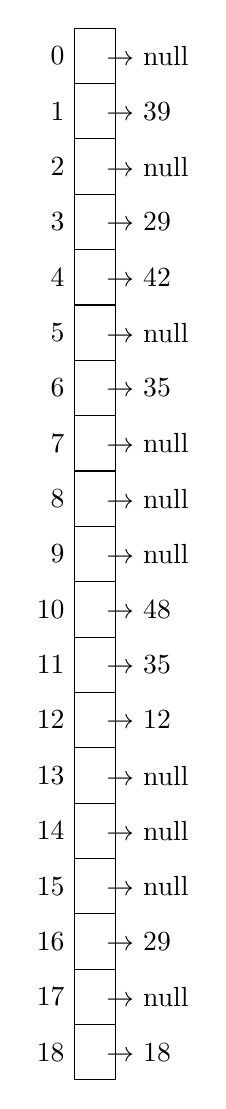
\begin{tikzpicture}
\coordinate (0);
\foreach \t[count=\i from 0,evaluate=\i as\j using int(\i+1)] in {
null,
39,
null,
29,
42,
null,
35,
null,
null,
null,
48,
35,
12,
null,
null,
null,
29,
null,
18
}
\node at(\i.south)[anchor=north,draw,minimum height=2em,minimum width=1.5em,outer sep=0pt](\j){}
    node at(\j.west)[align=right,left]{\i} 
    node at(\j.east)[align=left,right,xshift=-.7em]{$\rightarrow$ \t};
\end{tikzpicture}
\\
\textbf{Hash Table}
\\

\subsection{Size of the longest cluster}
The longest cluster has size of 3 at index 10, 11, and 12 consecutively.

\subsection{Number of occured collisions}
There were 10 collisions happened.

\subsection{Current load factor}
\begin{itemize}
    \item The table is an array of size 19 $\rightarrow$ N = 19
    \item Currently, there are 9 elements inside the hash table $\rightarrow$ n = 9
\end{itemize}
$\rightarrow$ \textit{The load factor = } $\frac{n}{N} = \frac{9}{19} \approx 0.47$